% =========================================================================== %

\begin{frame}[t,plain]
\titlepage
\end{frame}

% =========================================================================== %

\begin{frame}{Drinking Fountains}
%
\begin{columns}
\column{.5\linewidth}
\begin{center}
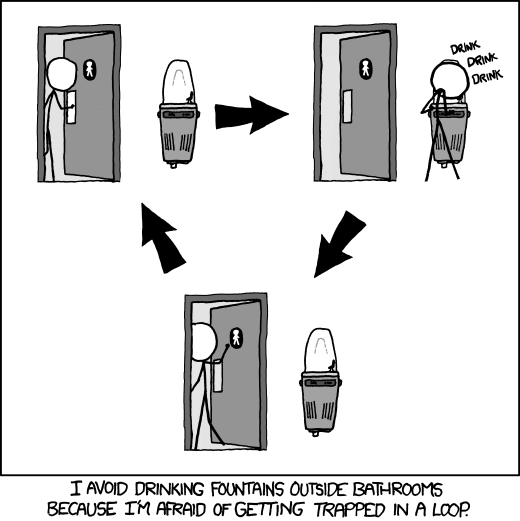
\includegraphics[width=.9\linewidth]{./gfx/08-xkcd-drinking-fountains}\\
\end{center}
%
\column{.4\linewidth}
\small
	\emph{\enquote{I've always wondered whether you could drink slowly enough, and eliminate fast enough, that you just sort of peed continuously.
		  But I'm afraid to try because I worry someone might call while I'm doing it and ask what I'm up to, and I won't be able to think of a lie.}}

	\vspace{6pt}
	\url{https://xkcd.com/986/}
\end{columns}
%
\end{frame}

% =========================================================================== %

\begin{frame}{Scope For Today}
%
\begin{itemize}
\item \inPy{for}-loops under the hood
	\begin{itemize}
	\item Iterables and Iterators
	\item The command \inPy{yield}
	\item Generator expressions
	\end{itemize}
\item Lazy Evaluation
	\begin{itemize}
	\item Short Circuiting
	\item \inPy{map} and \inPy{filter}
	\end{itemize}
\item The module \texttt{itertools}
\end{itemize}
%
\end{frame}

% =========================================================================== %

\begin{frame}[fragile]{Iterators and Iterables: Definition}
%
\begin{columns}
\column{.6\linewidth}
\begin{defbox}[Iterable]
An iterable is any instance of a class that provides an \inPy{__iter__} method which returns an iterator.
\end{defbox}
%
\begin{defbox}[Iterator]
An iterator is any instance of a class that privides an \inPy{__next__} method with either returns a value or raises \inPy{StopIteration}.
\end{defbox}
%
\column{.3\linewidth}

\includegraphics[width=\linewidth]{./gfx/08-geek}
\emph{So, everything's clear, right?}

\vspace{6pt}
\begin{flushright}
\tiny
\href{https://www.shutterstock.com/image-photo/beautiful-geek-woman-holding-digital-tablet-421481161}{Image Source: Shutterstock}
\end{flushright}
\end{columns}
%
\end{frame}

% =========================================================================== %

\begin{frame}[fragile]{Iterators and Iterables: \emph{Useful} Definitions}
%
\begin{defbox}[Iterable]
An iterable is any object that we loop over in a \inPy{for} loop. Examples include \inPy{list}s, \inPy{dict}s and file descriptors.
\end{defbox}
%
\begin{defbox}[Iterator]
An iterator is a temporary book keeping object that provides the means to find the next object or detect the end of the iterable when looping over it.
They are automatically generated in \inPy{for} loops.
\end{defbox}
%
\end{frame}

% =========================================================================== %

\begin{frame}[fragile]{In a Nutshell -- \inPy{for}-Loops Under the Hood}
%
\begin{itemize}
\item When running a \inPy{for}-loop, an iterator is automatically generated
\item This iterator is generated by the iterable
	\begin{itemize}
	\item \inPy{for} implies a call to the iterables \inPy{__iter__} method
	\item \inPy{__iter__} returns the iterator
	\item The presece of an \inPy{__iter__} method solely defines an iterable
	\end{itemize}
\item The iterator
	\begin{itemize}
	\item \enquote{knows} how to find the next object within the iterable
	\item reveals the next item via its \inPy{__next__} method
	\item raises \inPy{StopIteration} when the last element has been reached
	\item Each go through the loop calls \inPy{__next__} once
	\end{itemize}
\end{itemize}
%
\begin{hintbox}[Mixed Character]
\footnotesize
Usually, an iterator also has an \inPy{__iter__} method, \ie is an iterable itself. It usually just returns \inPy{self}.
\end{hintbox}
%
\end{frame}

% =========================================================================== %

\begin{frame}[fragile]
%
\begin{codebox}[The Code You Write]
\begin{minted}[fontsize=\footnotesize]{python3}
for element in iterable:
    ...
\end{minted}
\end{codebox}
%
\begin{codebox}[What Python Actually Does]
\begin{minted}[fontsize=\footnotesize]{python3}
iterator = iter(iterable)
while True:
    try:
        element = next(iterator)
        ...
    except StopIteration:
        break
\end{minted}
\end{codebox}
%
\begin{hintbox}[Magic Methods]
\footnotesize
\inPy{iter(iterable)} calls \inPy{iterable.__iter__}.\\
\inPy{next(iterator)} calls \inPy{iterator.__next__}.
\end{hintbox}
%
\end{frame}

% =========================================================================== %

\begin{frame}{So What's It Good For?}
%
\begin{itemize}
\item We can make our own class instances iterable
	\begin{itemize}
	\item E.\;g.: advanced data structures like trees
	\item E.\;g.: objects that only generate the next number in line without storing the entire sequence
	\item[\Thus] Possibly infinite sequences
	\end{itemize}
\item Standardized Interface makes own iterables compatible with a lot of Python-builtins and third-party libraries
	\begin{itemize}
	\item E.\;g. \inPy{min}, \inPy{max}, \inPy{sum}
	\item E.\;g. \inPy{list}, \inPy{tuple}
	\item E.\;g. \texttt{matplotlib.pyplot.plot} and \texttt{numpy.array}
	\end{itemize}
\end{itemize}
%
\end{frame}

% =========================================================================== %

\begin{frame}
%
\begin{columns}[T]
\column{.6\linewidth}
\begin{defbox}[Collatz Sequences]
\small
Let there be an arbitrary positive integer $c_0$. Then we can recursively define a sequence:
\begin{align*}
	c_{i+1} = \begin{cases}
	\dfrac{1}{2}c_i & \text{if~} c_i \text{~even}\\
	3 c_i + 1 & \text{otherwise}
	\end{cases}
\end{align*}
\end{defbox}
%
\begin{hintbox}[The Collatz Conjecture]
\small
The Collatz conjecture states that, for any integer $c_0$, this sequence will eventually arrive at a loop $1 \to 4 \to 2 \to 1 \to ...$

Introduced in 1937, it is one of the most famous \emph{unsolved} problems in mathematics.\\
(\Thus \emph{Don't waste your time on it.})
\end{hintbox}
%
\column{.3\linewidth}
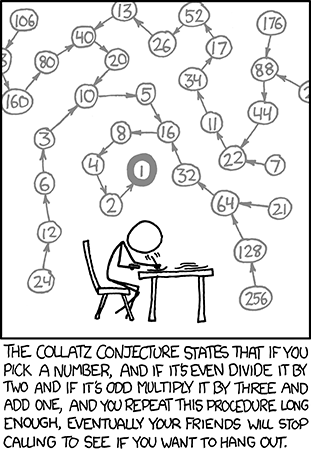
\includegraphics[width=.9\linewidth]{./gfx/08-xkcd-collatz}

\footnotesize
\emph{The Strong Collatz Conjecture states that this holds for any set of obsessively-hand-applied rules."}\\
\url{https://xkcd.com/710/}
\end{columns}
%
\end{frame}

% =========================================================================== %

\begin{frame}[fragile]
%
\begin{columns}[T]
\column{.7\linewidth}
\begin{codebox}[A Collatz Sequence Generator]
\begin{minted}[fontsize=\footnotesize, linenos]{python3}
class Collatz:
    def __init__(self, n):
        self.n = 2 * n

    def __iter__(self):
        return self

    def __next__(self):
        if self.n % 2 == 0:
            self.n = self.n // 2
        else:
            if self.n == 1: raise StopIteration
            self.n = 3 * self.n + 1
        return self.n

for num in Collatz(9):
    print(num)
\end{minted}
\end{codebox}
%
\column{.2\linewidth}
\begin{cmdbox}[Output]
\begin{minted}[fontsize=\footnotesize]{text}
9   13
28  40
14  20
7   10
22  5
11  16
34  8
17  4
52  2
26  1
\end{minted}
\end{cmdbox}
%
\footnotesize
\emph{Read column-wise. Output has been wrapped to fit on this slide.}
\end{columns}
%
\end{frame}

% =========================================================================== %

\begin{frame}
%
\begin{hintbox}[Consuming Iteration]
The above example \emph{changes the state} of the iterable in each iteration. In other words, the iterable is consumed, it can only be used once. This is not uncommon, as it is computationally cheap to (re)create a fresh iterable, and this single-use approach spares the effort of using a lot of memory.
\end{hintbox}
%
\begin{hintbox}[Example: Tree Structure]
See GRIPS for a more involved example that shows how to build and store a tree structure (on the example of a file system) and how to iterate over the tree.

\vspace{6pt}
True to the nature of a tree as a \emph{self similar structure}, this example also helps you to refresh your skills in \emph{recursive algorithms}.
The actual iterator, however, is implemented in a non-recursive manner.
\end{hintbox}
%
\end{frame}

% =========================================================================== %

\begin{frame}[fragile]{Cutting Down to the Essential Bits -- the Command \inPy{yield}}
%
\begin{itemize}
\item Can be used in regular functions
\item Like \inPy{return}: leave function and report value to calling site
\item But: resuming the function (as opposed to restarting) at the next call
	\begin{itemize}
	\item Restarting: all variables in the function are reset
	\item Resuming: the previous values of the function and even the line in which we left it are preserved
	\end{itemize}
\item Think of this as implicitly generating a class with \inPy{__iter__} and \inPy{__next__}
\item The function result becomes an iterable
	\begin{itemize}
	\item More precisely: \emph{generator object}
	\item Actually has \inPy{__iter__} and \inPy{__next__}
	\item End of iteration not by \inPy{raise StopIteration}, but simply by exiting the function (\inPy{return None} or going beyond the last code line of the function)
	\end{itemize}
\item Changing internal state of function \Thus consuming iteration
\end{itemize}
%
\end{frame}

% =========================================================================== %

\begin{frame}[fragile]
%
\begin{codebox}[A Generator Function]
\begin{minted}[fontsize=\footnotesize, linenos]{python3}
def collatz(n):
    yield n
    while n != 1:
        if n % 2 == 0: n //= 2
        else:          n = 3 * n + 1
        yield n

for num in Collatz(9):
    print(num)
\end{minted}
\end{codebox}
%
Output: \emph{Same as the previous example}
%
\begin{hintbox}[Short-Form for Consumable Iterables]
When implementing a consumable sequence, \inPy{yield} allows to focus on the interesting bits.
\end{hintbox}
%
\end{frame}

% =========================================================================== %

% Generator Expressions